\documentclass[12pt,letterpaper,final]{article}

\usepackage{Sweave}
\usepackage{graphicx}
\usepackage{natbib}
\usepackage{hyperref}
\usepackage{caption}
\usepackage{rotating}
\usepackage{verbatim}
\usepackage{textcomp}
\usepackage{wasysym}

\setlength{\oddsidemargin}{0in}
\setlength{\textwidth}{6.15in}
%\setlength{\topmargin}{0.5in}
\setlength{\textheight}{22cm}
\setlength{\headheight}{0in}
\setlength{\headsep}{0in}
\setlength{\parskip}{5pt plus 2pt minus 3pt}

\def\thefootnote{\fnsymbol{footnote}}
\setcounter{footnote}{1}

\renewcommand{\baselinestretch}{1.2}
\renewcommand{\labelenumi}{(\roman{enumi})}

\renewcommand{\topfraction}{1.0}
\renewcommand{\bottomfraction}{1.0}
\renewcommand{\textfraction}{0.0}
\renewcommand{\floatpagefraction}{1.0}

\newtheorem{definition}{Definition}
\newtheorem{theorem}{Theorem}
\newtheorem{lemma}[theorem]{Lemma}
\newtheorem{claim}[theorem]{Claim}
\newtheorem{fact}[theorem]{Fact}

% to get nice proofs ...
\newcommand{\qedsymb}{\mbox{ }~\hfill~{\rule{2mm}{2mm}}}
\newenvironment{proof}{\begin{trivlist}
\item[\hspace{\labelsep}{\bf\noindent Proof: }]
}{\qedsymb\end{trivlist}}


\newfont{\msymb}{cmsy10 scaled 1000}

\def\nullset{\mbox{\O}}
\def\R{{I\!\!R}}
\def\C{{I\!\!\!\!C}}
\def\N{{I\!\!N}}

\def\P{\mbox{\msymb P}}


%\parskip 0.1in
\pagenumbering{arabic}    %  Start using 1,2,... as page numbers.
\pagestyle{plain}         %  Page numbers in middle bottom of page.
%\setcounter{page}{80}  % XXXXXXXXXXXXXXXXX
%\setcounter{theorem}{5} % XXXXXXXXXXXXXXXXX
%\setcounter{definition}{10} % XXXXXXXXXXXXXXXXX

\parindent 0in


\begin{document}

\Sconcordance{concordance:hw01_blank.tex:hw01_blank.Rnw:%
1 142 1 1 2 1 0 2 1 3 0 1 2 5 1 1 4 17 1 1 4 4 1 1 4 3 1 1 4 18 1 1 4 %
16 1 1 4 7 1 1 4 18 1 1 4 10 1 1 4 18 1 1 4 18 1 1 4 61 1}


\begin{titlepage}
\vspace*{4.5cm}
\begin{center}
{\LARGE \bf Stat 5810, Section 003} \\[0.5cm]
{\LARGE \bf Statistical Visualization I} \\[0.5cm]
{\LARGE \bf Fall 2018} \\[0.5cm]
{\LARGE \bf Homework 1} \\[0.5cm]
~ \\[2cm]
{\bf ShaunMicheal Bartschi} \\[0.3cm]
{A01975136} \\[0.3cm]
{October 17, 2018} \\[0.3cm]
\end{center}

\thispagestyle{empty}
\vfill
\end{titlepage}


\begin{table}\centering
\begin{tabular*}{6.15in}{@{\extracolsep{\fill}}|llr|} \hline
Stat 5810 Statistical Visualization I & \hspace*{0.5 in} & Fall 2018 \\
 & & \\
\multicolumn{3}{|c|}{
Homework Assignment 1 (10/6/2018)} \\
 & & \\
\multicolumn{3}{|c|}{
60 Points --- Due Wednesday 10/17/2018 (via Canvas by 11:59pm)} \\
\hline
\end{tabular*}
\end{table}


\begin{enumerate}

\item (48 Points)
In this question, you have to work with the {\it Hidalgo1872.rda} data set
that is provided in Canvas. You can also directly download the data from 
\url{https://github.com/cran/MMST/tree/master/data}.
Do not use any other version of this data set you may find on the
internet
or your results may differ slightly as different versions
of the data set seem to exist. This data set was
originally a part of the {\it MMST} R package, but that
package was removed from the CRAN repository. 

The data set consists of 485 rows and 3 columns. The first column
({\it thickness}) contains the thickness of 485 Mexican stamps,
measured to a precision of a thousandth of a millimeter.
It is my understanding that 
column 2 ({\it thicknessA}) repeats these measurements if the stamp was pressed in 1872
(and contains NA otherwise). 
Column 3 ({\it thicknessB}) repeats these measurements if the stamp was pressed in 1873/74
(and contains NA otherwise). 
There are a few data entry errors where both columns 2 and 3 contain 
a measurement.

The full (?!?) description of the data set, as originally provided
in the {\it MMST} R package, is shown in Figure~\ref{Hidalgo1872}.


\begin{figure}[ht]
\centering{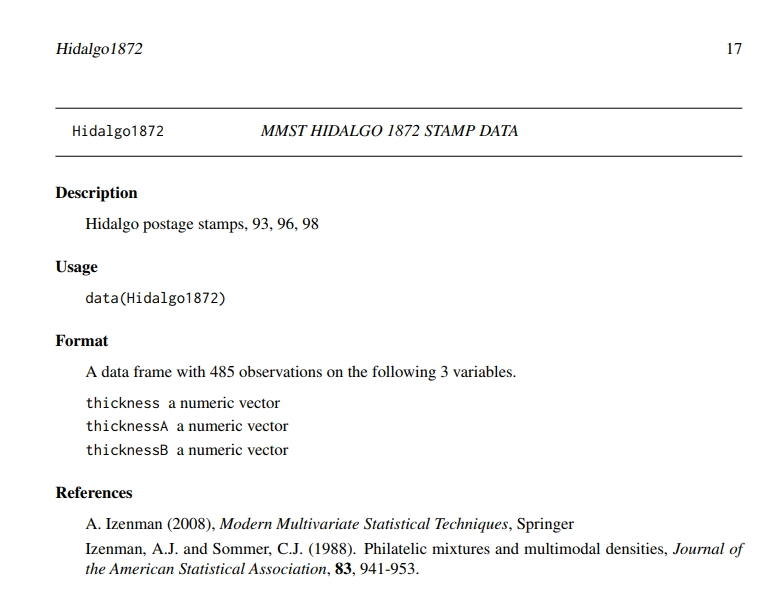
\includegraphics[width=4.3in]{Hidalgo1872.jpg}}
\caption{\label{Hidalgo1872}
Description of the Hidalgo 1872 data set, obtained from 
\url{https://mran.microsoft.com/snapshot/2014-09-30/web/packages/MMST/MMST.pdf}.
}
\end{figure}



\begin{enumerate}
\item (1 Point) 
Load the Hidalgo1872 data set and
all required R packages to answer this question. Show your R code.

\begin{Schunk}
\begin{Sinput}
> setwd("C:/Users/Shaun/Desktop/StatVis/HW1")
> load("Hidalgo1872.rda")
> library(ggplot2)
\end{Sinput}
\end{Schunk}


\item (2 Points) 
Draw a basic histogram for {\it thickness} using ggplot2.
Include your R code and the resulting graph.



\item (6 Points) 
Further improve your histogram from (b). 
Try three different binwidths: 0.001, 0.002, and 0.005 and use 0.0005, 0.001, and 0.0025
as the center, respectively.
You should also adjust the
range of the horizontal and vertical axes, labels, title, etc. 
{\bf Clearly indicate which changes
you made and why you made these changes.}
As in class, make these changes step by step and continue with further
adjustments until your graph is ready for publication.
Include your three final graphs for these three binwidths and the R code
for these finals graph. No need to include any intermediate graphs and the R code for those.
Hint: When you get warnings from ggplot2, check carefully. It is easy to cut off
parts of the histogram on the horizontal or vertical axis, in particular when
you copy and paste your R code and forget to adjust some of the arguments.



\item (1 Point) 
Repeat (b) from above, now using the {\it hist} function from baseR.



\item (6 Points) Repeat (c) from above, now using the {\it hist} function from baseR.



\item (4 Points)
Based on your final histograms in (c) and (e), how many modes does the Hidalgo 1872 data set
seem to have? Answer this question separately for your three different binwidths.
What is your overall conclusion regarding the number of modes?


\item (4 Points)
Recall that the stamps originate from the years 1872 and 1873/74. The help page shown in
Figure~\ref{Hidalgo1872} is not very helpful, so we have to make our own assumptions:
If the third column ({\it  thicknessB}) contains a value, then this is a measurement
from 1873/74. Otherwise, it is a measurement from 1872. Using any approach in R you are
familiar with, add a column called {\it Year} to the Hidalgo1872 data frame.
You cannot modify the data outside of R, e.g., via Excel. Show your R code,
the first 6 lines of your modified data frame, and a table that summarizes
the new {\it Year} column. Hint: There should be 289 measurements for 1872
and 196 for 1873/74.



\item (6 Points)
Start with a basic histogram for {\it thickness}, conditioned on the
two options for {\it Year}, using ggplot2. Optimize this graph
in multiple steps. Use a layout that shows the two resulting
histograms above each other for better comparison.
As before,
try three different binwidths: 0.001, 0.002, and 0.005 and use 0.0005, 0.001, and 0.0025
as the center, respectively.
Include your R code and the resulting final figure
that consists of six histograms overall: 1872 on top and 1873/74 at the bottom and binwidths
0.001, 0.002, and 0.005 from left to right. The two histograms above each other
should follow the small multiple principle, i.e., have the same ranges for the
horizontal and vertical axes. The histograms besides each other do not
have to follow this principle



\item (6 Points) 
Repeat (h) from above, now using the {\it hist} function from baseR.
In particular, use the same layout as described above.
Hint: Now you have to be really careful to use the proper ranges
for the horizontal and vertical axes.



\item (4 Points)
Based on your final histograms in (h) and (i), how many modes does the Hidalgo 1872 data set
seem to have for each year? Answer this question separately for your two different years
(1872 and 1873/74) and your three different binwidths.
What is your overall conclusion regarding the number of modes?


\item (4 Points) Would boxplots be good replacements for the two histograms
for the two years? Compare carefully what can be seen in the box plots
and what cannot be seen.
First create two basic boxplots with a package of your choice. Then refine them.
Add labels as needed and make sure your boxplots follow the
small multiple principle.
As always, include your R code and the final resulting graphs.
Then answer {\bf yes} (they are good replacements) or {\bf no}
(they are not good replacements). Justify your answer!



\item (4 Points) Have you ever heard of violin plots? If not, google them!
Find a suitable R package that creates violin plots or see how they can be
created in ggplot2.
Would violin plots be good replacements for the two histograms? 
First create two basic violin plots with a package of your choice.
As always, include your R code and the final resulting graphs.
Then answer {\bf yes} (they are good replacements) or {\bf no}
(they are not good replacements). Justify your answer!


\end{enumerate}


\newpage


\item (12 Points)
This question makes use of the {\it Pima.tr2} data set 
from the {\it MASS} R package again.
These graphs may not be perfect and may need some
further adjustments, but those are not required to get full points in this question.


\begin{enumerate}
\item (6 Points) Recreate the graphs (and layout) shown in Figure~\ref{hw01_q2b} using baseR.
Include your R code and the resulting graphs.
Hint: You can create a new line via \verb|\n| without any extra spaces before/after \verb|\n|.



\begin{figure}[ht]
\centering{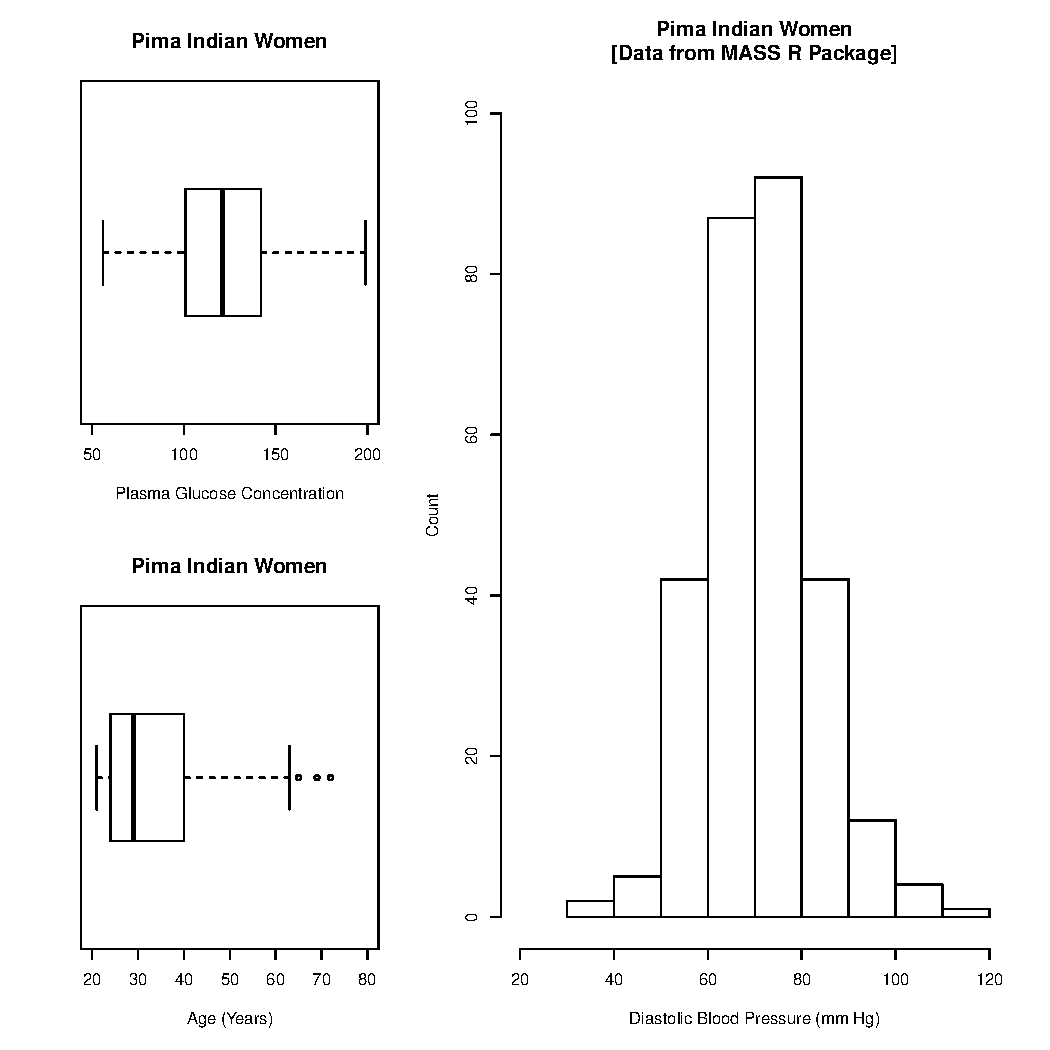
\includegraphics[width=6.0in]{hw01_q2a.pdf}}
\caption{\label{hw01_q2a}
Graphs created with baseR.
}
\end{figure}


\newpage


\item (6 Points) Recreate the graph shown in Figure~\ref{hw01_q2b} using ggplot2.
Include your R code and the resulting graph. Note: You have to
change some of the labels and adjust the grid lines so they do not 
run through the middle of some of your bars. Find suitable help pages or
information on stackoverflow.



\begin{figure}[ht]
\centering{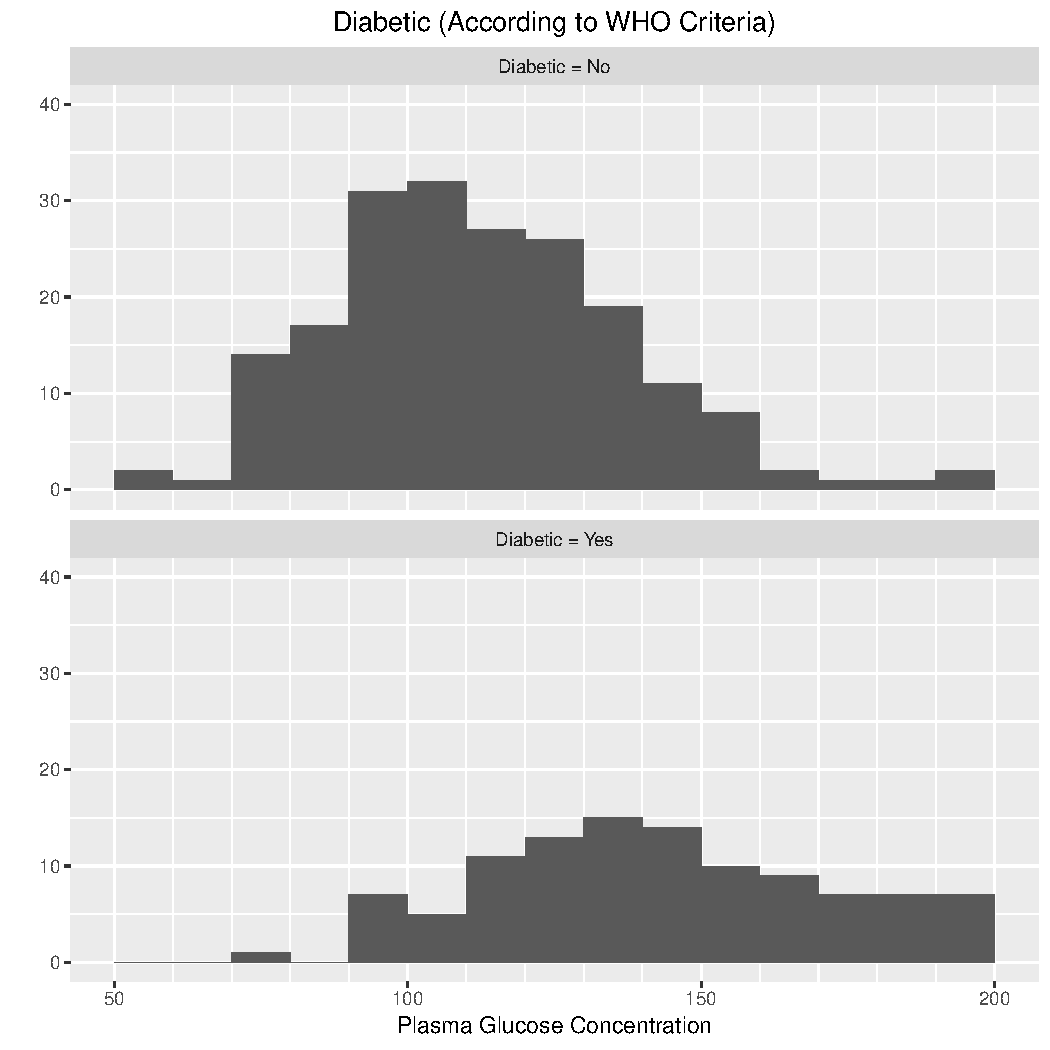
\includegraphics[width=6.0in]{hw01_q2b.pdf}}
\caption{\label{hw01_q2b}
Graph created with {\it ggplot2}.
}
\end{figure}


\end{enumerate}

\end{enumerate}


\newpage


\noindent{\Large \bf General Instructions}~\\


\begin{enumerate}
\item Create a single html or pdf document, using R Markdown, Sweave, or knitr.
You only have to submit this one document.

\item Include a title page that contains your name, your A-number, the number of
the assignment, the submission date, and any other relevant information.

\item Start your answers to each main question on a new page (continuing with the next
part of a question on the same page is fine). 
Clearly label each question and question part.

\item Before you submit your homework, check that you
follow all recommendations from Google's R Style Guide
(see \url{https://google.github.io/styleguide/Rguide.xml}). 
Moreover, make sure that your R code is consistent, i.e., that you use the same
type of assignments and the same type of quotes throughout your entire homework.

\item Give credit to external sources, such as stackoverflow or help pages. Be specific
and include the full URL where you found the help (or from which help page you got 
the information). Consider R code from such sources as ``legacy code or third-party code'' 
that does not have to be adjusted to Google's R Style (even though it would be nice,
in particular if you only used a brief code segment).

\item {\bf Not following the general instructions outlined above will result in point deductions!}

\item For general questions related to this homework, please
use the corresponding discussion board in Canvas! I will try to
reply as quickly as possible. Moreover, if one of you knows
an answer, please post it. It is fine to refer to web pages
and R commands, but do not provide the exact R command with all required arguments
or which of the suggestions from a stackoverflow web page eventually worked for you! 
This will be the task for each individual student!

\item Submit your single html or pdf file via Canvas by the submission deadline.
Late submissions will result in point deductions as outlined on the syllabus.

\end{enumerate}


\end{document}

